\section{Implementace}

\subsection*{Konkrétní rozdělení práce v tůmu}
\begin{itemize}
    \item[] Ondřej Fojt     - administrativní pracovník
    \item[] Vít Hrbáček     - Fyzioterapeut
    \item[] Vladimír Mečiar - Pacient
\end{itemize}

\subsection*{Popis použitých nástrojů}
    knihovna JQuery pro jednodušší práci s javascriptem


\subsection*{Popis implementace}

\subsubsection*{Administrativní pracovník}

Celá sekce pro administrativního pracovníka je implementována v rámci jednoho html souboru, ve kterém se schovávají a objevují prvky.
Všechna komunikace s BE je prováděna asynchronně a to funkcí \hyperlink{https://api.jquery.com/jQuery.getJSON/}{jQuery.getJSON( url [, data ] [, success ] )}.

Na všech zobrazeních lze přepínat datum po dnech s výjimkou kalendáře, kde se posouvá po celém týdnu.
Po kliknutí na službu v rámci grafu vytíženosti se zobrazí 2 další grafy pro danou službu. Tyto grafy reprezentují vytíženost zaměstnanců pro danou službu a vytíženost celé služby(všech zaměstnanců) sepsané po dnech(počet následujících dní je omezen pouze počtem vracených dat na BE).
V rámci grafu vytíženosti zaměstnanců a v seznamu zaměstnanců jsou odkazy na kalendář, kde se zobrazují konkrétní registrace.
Graf vytíženosti mění svůj význam podle výběru, tedy pokud se zvolila konkrétní služba tak se zobrazuje Vytíženost zaměstnanců v rámci služby v jeden den a vytíženost služby po dnech.
Vyhledávání na úvodní stránce by mělo vyhledávat služby, zaměstnance a pacienty, ale je pouze implementované vyhledávání služeb.
V kalendáři se lze po kliknutí na registraci zobrazení její detaily.
Měla by být možnost přidávat a odebírat(potažmo přesunout) registrace, ale toto není implementováno.
Zásobník akcí pro undo, není bohužel implementován, ale tlačítkem domů v levém horním rohu se lze vrátit na počáteční stránku.

Stránky administrativního pracovníka lze prohlížet \hyperlink{https://www.stud.fit.vutbr.cz/~xfojto00/ITU/adm_wkr/}{zde}.


\subsubsection*{Fyzioterapeut}

Rozhraní určené pro pracovníky Fyzioterapeutického oddělení, fyzioterapeuty, bylo vytvořeno v oddělené a současně samostatné jednotce 
HTML souboru, ind.html. Kód byl sestaven z prvků v jazycích HTML, CSS a JavaScript. Prvek HTML tabulky byl využit pro tvorbu rozvrhu, 
CSS šablona je určena například k tomu,  aby jednotlivé prvky dala na jejich pozice nebo zajišťuje, že každý sudý sloupec tabulky má jinou barvu.
Sekce JavaScriptového kódu slouží k načtení dat z backendu pro splnění podle pravidel pro MVC. Program kontroluje každé dvě sekundy zda se rozvrh 
nezměnil. Dvě sekundy jsme v týmu zvolili jako rozumnou dobu, kdy nemusí uživatel moc čekat, ale současně zároveň má velmi aktuální rozvrh. 
Pro zajištění komunikace s daty v backendové části jsme použili asynchronní komunikaci stejnou jako byla na cvičení.

Stránky fyzioterapeuta lze prohlížet \hyperlink{http://iturezervacnisystem.wz.cz/ind.html}{zde}.

\subsubsection*{Pacient}


\section*{Výsledná aplikace}

\subsection{Administrativní pracovník}

\begin{figure}[htbp]
    \centering
    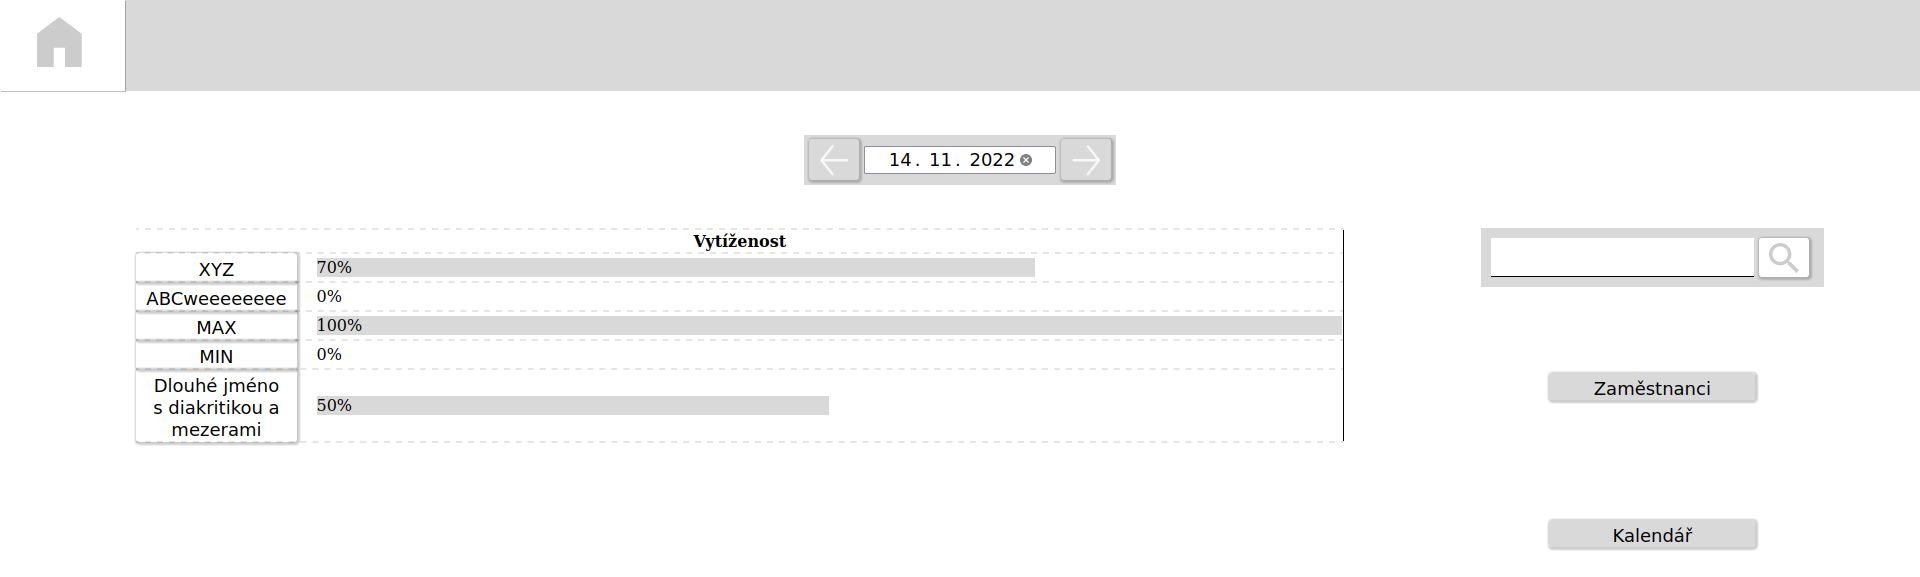
\includegraphics[angle=0, origin=c, width = \textwidth]{doc/latex/fig/implementation/admin/main_page.png}
    \caption{Hlavní stránka administrativního pracovníka}
\end{figure}

\begin{figure}[htbp]
    \centering
    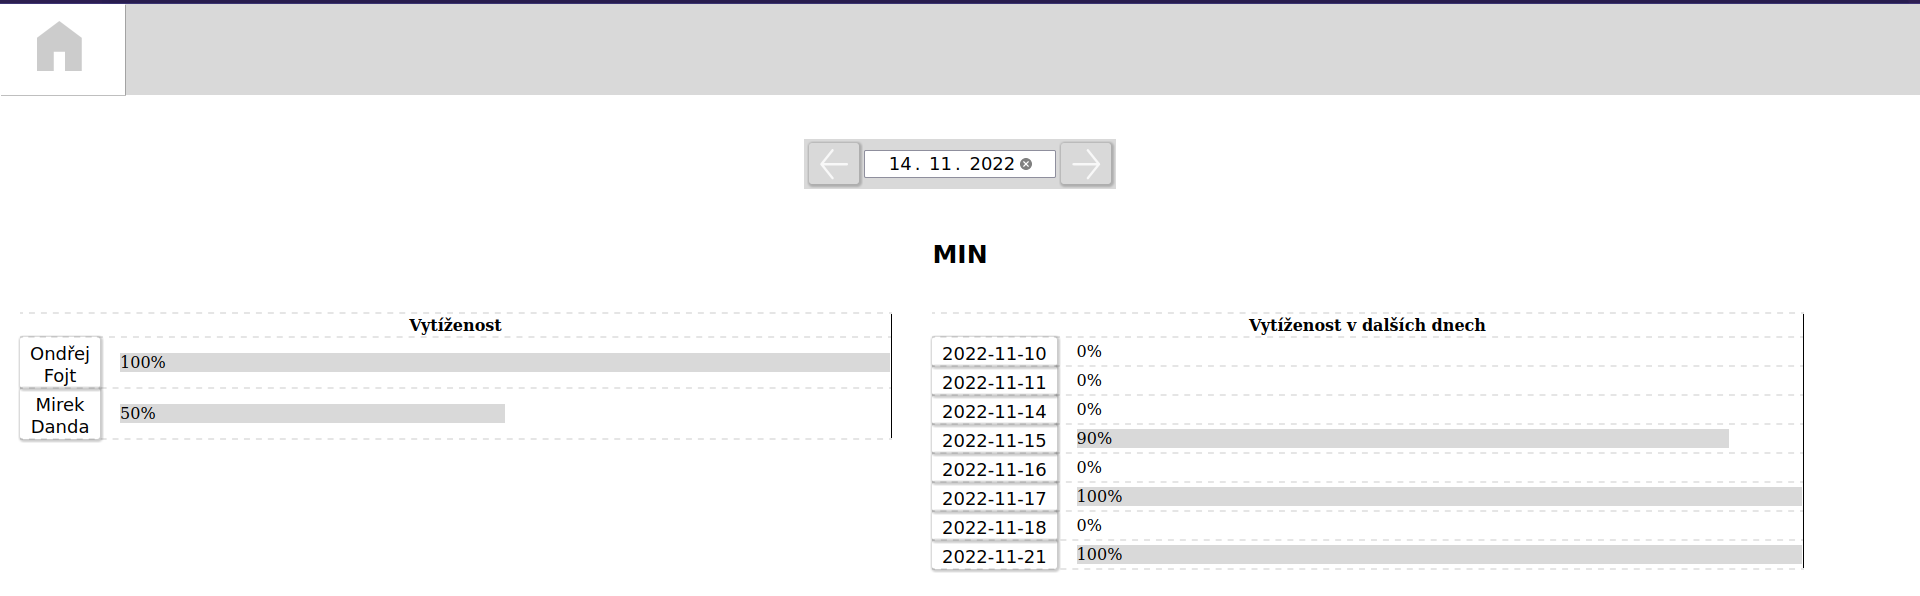
\includegraphics[angle=0, origin=c, width = \textwidth]{doc/latex/fig/implementation/admin/service.png}
    \caption{Grafy zaplněnosti pro danou službu}
\end{figure}

\begin{figure}[htbp]
    \centering
    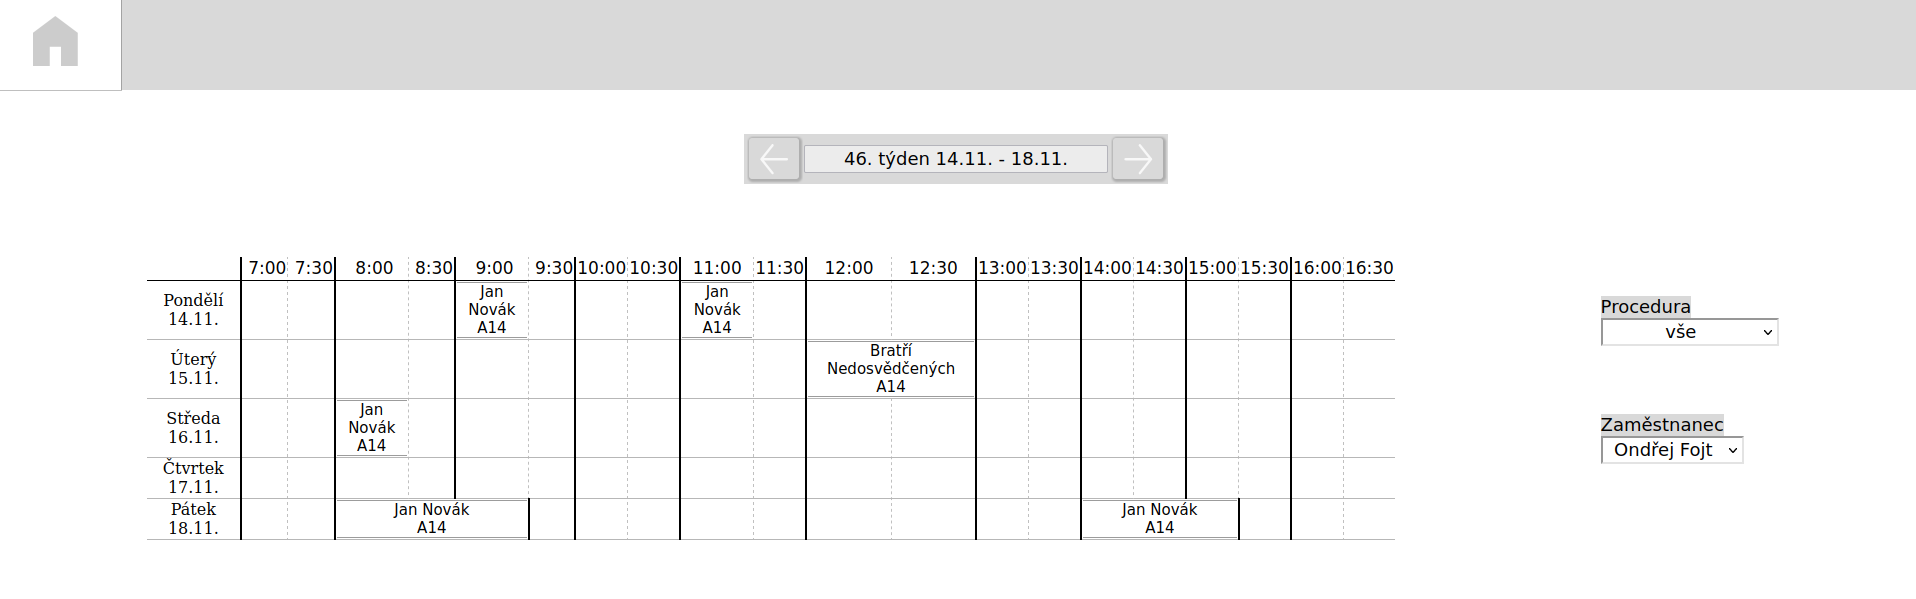
\includegraphics[angle=0, origin=c, width = \textwidth]{doc/latex/fig/implementation/admin/calendar.png}
    \caption{Kalendář služeb/procedur}
\end{figure}



\begin{figure}[htbp]
    \centering
    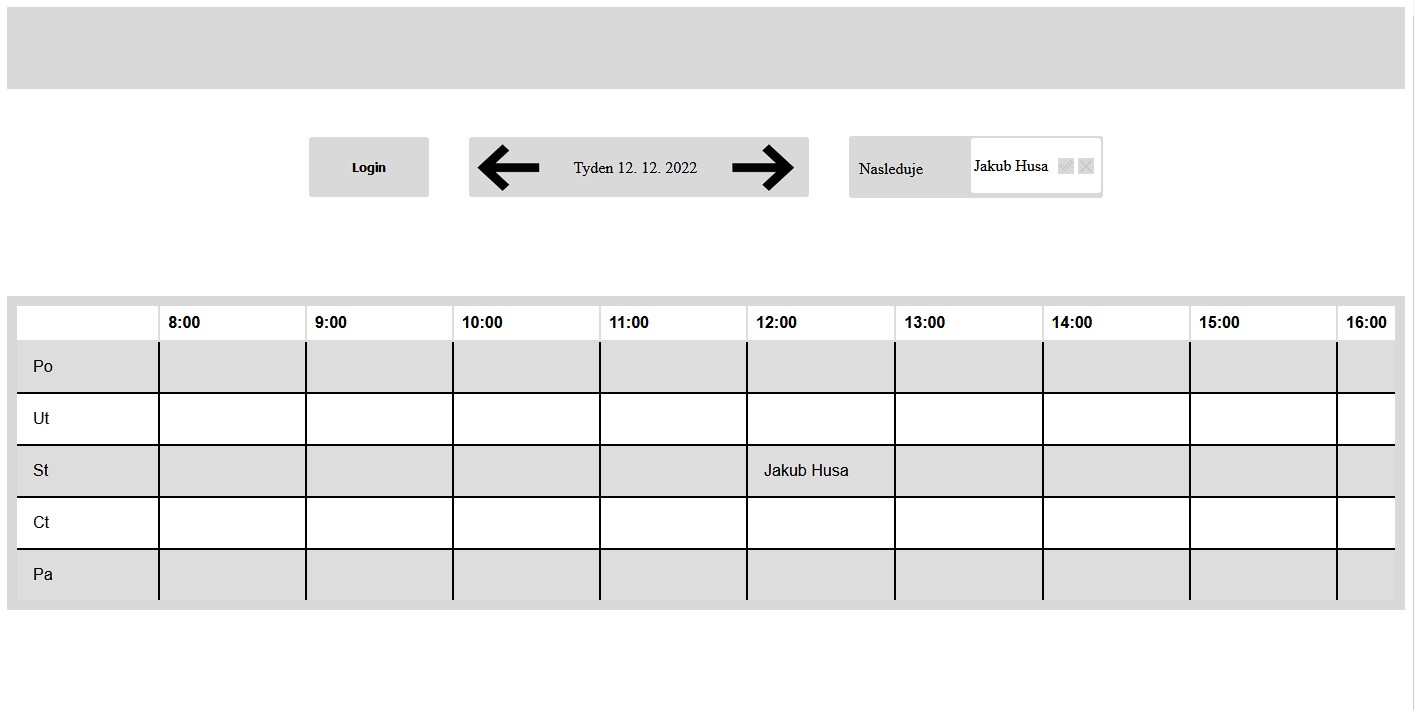
\includegraphics[angle=0, origin=c, width = \textwidth]{doc/latex/fig/implementation/fyzio/printscreen_fyzio.jpg}
    \caption{Stránka fyzioterapeuta}
\end{figure}
